% Preamble
\documentclass[11pt, presentation]{beamer}
%\usetheme{warsaw}
%\usetheme{madrid}
\usetheme{metropolis}
\setbeamerfont{caption}{size=\scriptsize}
\AtBeginSection[]{
    \begin{frame}[standout]
	\insertsectionhead
        %\vfill
        %\centering
       % \begin{beamercolorbox}[sep=8pt,center,shadow=true,rounded=true]{title}
        %    \usebeamerfont{title}\insertsectionhead\par%
        %\end{beamercolorbox}
      %  \vfill
    \end{frame}
}
\setbeamerfont{bibliography item}{size=\footnotesize}
\setbeamerfont{bibliography entry author}{size=\footnotesize}
\setbeamerfont{bibliography entry title}{size=\footnotesize}
\setbeamerfont{bibliography entry location}{size=\footnotesize}
\setbeamerfont{bibliography entry note}{size=\footnotesize}


\title{Image Super Resolution}
\author{Ali Ghanbari}
%\institute[Inst.]{K. N. Tossi University}
\date{November 28, 2022}
\titlegraphic{
    
\includegraphics[width=3cm]{images/kntu-logo-r1}
}


% Packages
\usepackage{amsmath}
\usepackage{graphicx}
\usepackage{xcolor}
\usepackage{beamerbasetitle}
\usepackage{subfiles}

% Document
\begin{document}
%    \maketitle
    \begin{frame}
        \centering
        
\includegraphics[width=2cm]{images/kntu-logo-r1}
        \vfill
        \textbf{\Large Overview of Image Super Resolution Methods}
        \vfill
        Professor: Dr. Farnaz Sheikhi

        Presenter: Ali Ghanbari
        \vfill
        \small November 28, 2022
    \end{frame}
    \begin{frame}{Overview}
        \begin{enumerate}
            \item Introduction
            \item Applications
            \item Evaluation Index
            \item Datasets
	 \item Methods
            \item Interpolation Based Methods
            \item CNN Based Methods
            \item GAN Based Methods
            \item Conclusion
        \end{enumerate}
    \end{frame}
    \begin{frame}
        \frametitle{Introduction}
        Image super-resolution reconstruction refers to a technique of recovering
        a high-resolution (HR) image from a low-resolution (LR) degraded image~\cite{li2020}

        \begin{figure}
            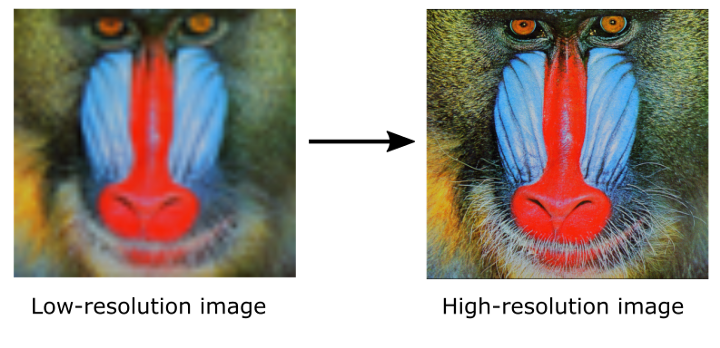
\includegraphics[width=0.75\textwidth]{images/sisr}
            \caption{Transform your low-resolution images to high-resolution images~\cite{bhsri}}
            \label{fig:sisr}
        \end{figure}
    \end{frame}
    \begin{frame}
        \frametitle{Applications}
        Image super resolution is popularly used in the following applications~\cite{psrsisr}:
        \begin{itemize}
            \item Surveillance
            \item Medical
            \item Media
        \end{itemize}
    \end{frame}
    \begin{frame}
        \frametitle{Datasets}
        A lot of different datasets available for training and testing super resolution models.

        Popular training datasets:
        \begin{itemize}
            \item \href{ http://www.ifp.illinois.edu/~jyang29/codes/ScSR.rar}{91 Image}
            \item\href{ https://www2.eecs.berkeley.edu/Research/Projects/CS/vision/grouping/segbench/BSDS300-images.tgz}{BSD300} 
            \item\href{http://cv.snu.ac.kr/research/EDSR/Flickr2K.tar}{Flickr2K}
        \end{itemize}
        Popular testing datasets:
        \begin{itemize}
            \item \href{http://people.rennes.inria.fr/Aline.Roumy/results/SR_BMVC12.html}{Set5}
            \item\href{https://github.com/jbhuang0604/SelfExSR}{Set14}
            \item \href{https://sites.google.com/site/jbhuang0604/publications/struct_sr}{Urban100}
        \end{itemize}
%        \begin{figure}
%            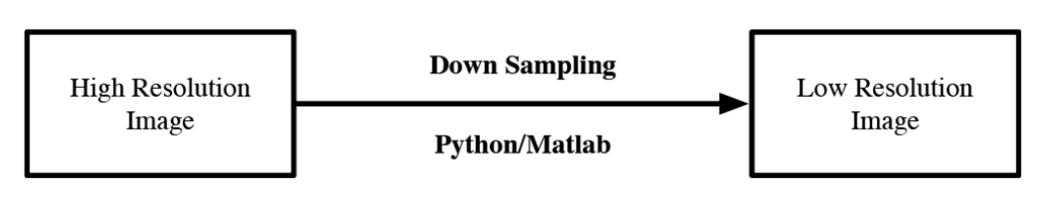
\includegraphics[width=0.75\textwidth]{images/lr}
%            \caption{Flowchart of LR image acquisition}
%            \label{fig:lr}
%        \end{figure}
    \end{frame}
    \begin{frame}
        \frametitle{Evaluation Index}
        Current mainstream objective evaluation methods:
        \begin{itemize}
            \item Peak signal to noise ratio (PSNR)
            \item Structural similarity (SSIM)
            \item Perceptual index (PI)
            \item Root MSE (RMSE)
        \end{itemize}
    \end{frame}
    \begin{frame}
        \frametitle{Methods}
        Some of the methods that we are going to look at:
        \begin{itemize}
            \item Based on Interpolation
            \item Based on CNN
            \item Based on GAN
        \end{itemize}
    \end{frame}
    \begin{section}{Interpolation Based Methods}
        \begin{frame}
            \frametitle{Interpolation}
            Interpolation works by using known data to estimate values at unknown points.
            \begin{figure}
                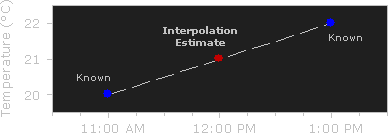
\includegraphics[width=0.6\textwidth]{images/interpolation_graph1}
                \caption{Linear interpolation for temperature at noon~\cite{camii}}
                \label{fig:interpolation-linear}
            \end{figure}
        \end{frame}
        \begin{frame}
            \frametitle{Image Interpolation}
            Image interpolation works in two directions, and tries to achieve a best approximation of a pixel's color and intensity based on the values at surrounding pixels.
            \begin{figure}
                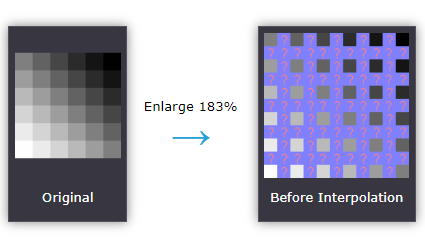
\includegraphics[width=0.75\textwidth]{images/image-interpolation}
                \caption{How resizing / enlargement works~\cite{camii}}
                \label{fig:img-interpolation}
            \end{figure}
        \end{frame}
        \begin{frame}[label=interpolation]
            \frametitle{Interpolation Methods}
            List of interpolation algorithms:
            \begin{itemize}
                % https://www.cambridgeincolour.com/tutorials/image-interpolation.htm
                \item Nearest Neighbor Interpolation
                \item Bilinear Interpolation
                \item Bicubic Interpolation
                \item Method based on Directional Bicubic Interpolation
                \item Method based on DWT and BI
            \end{itemize}
        \end{frame}
        \begin{frame}
            \frametitle{Bicubic Interpolation}
            Bicubic considers the closest 4x4 neighborhood of known pixels — for a total of 16 pixels.
            Since these are at various distances from the unknown pixel, closer pixels are given a higher weighting in the calculation.
            Compared to previous methods it:
            \begin{itemize}
                \item Produces Sharper Images
                \item Offers a Balance Between Time and Output Quality
                \item is the Standard Method Used in Many Image Editing Programs
            \end{itemize}
            \only<2->{However it only
            interpolates the image edges horizontally and vertically so that the
            edges are vulnerable to artifacts.}
        \end{frame}
        \begin{frame}
            \frametitle{Interpolation Artifacts}
            All non-adaptive interpolators attempt to find an optimal balance between three undesirable artifacts: edge halos, blurring and aliasing.
            \begin{figure}
                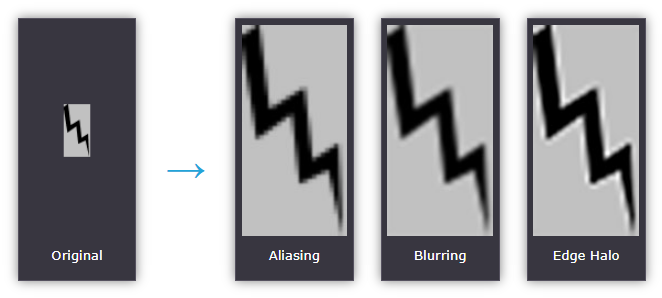
\includegraphics[width=0.75\textwidth]{images/interpolation-artifacts}
                \caption{Image interpolation Artifacts~\cite{camii}}
                \label{fig:artifacts}
            \end{figure}
        \end{frame}
        \begin{frame}
            \frametitle{Method based on Directional Bicubic Interpolation}
            \begin{columns}
                \begin{column}{0.5\textwidth}
                    This methods interpolates
                    lost pixels based on local intensity and direction to better preserve
                    sharp edges and details.
                \end{column}
                \begin{column}{0.5\textwidth}
                    \begin{figure}
                        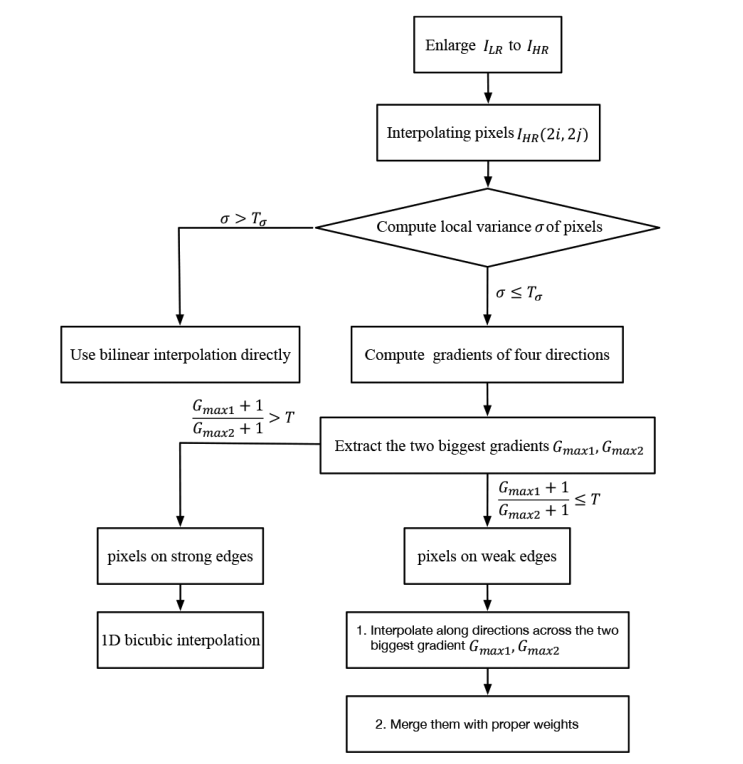
\includegraphics[width=\textwidth]{images/bi-method}
                        \caption{Flowchart of directional BI method}
                        \label{fig:dbi-method}
                    \end{figure}
                \end{column}
            \end{columns}
        \end{frame}
        \begin{frame}
            \frametitle{Method based on DWT and BI}
            \only<1>{
                a super-resolution technique based on the interpolation of
                high-frequency sub-band images obtained by the discrete wavelet
                transform (DWT) and input images.
            }
            \only<2>{
                Signal filters used on the image:
                \begin{itemize}
                \item HPF (High Pass Filter)- to extract edges
                \item LPF (Low Pass Filter)-for approximation
                \end{itemize}
            }
            \only<3>{
                The image is decomposes into 4 sub-band:
                \begin{itemize}
                \item LL — gives an approximation
                \item LH — Horizontal features (HPF along rows)
                \item HL — Vertical features(HPF along col.)
                \item HH — Diagonal features
                \end{itemize}
            }
            \only<1-3>{
                \begin{figure}
                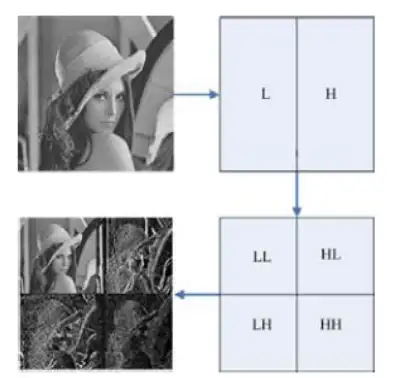
\includegraphics[width=0.4\textwidth]{images/dwt}
                \caption{Discrete wavelet transform(DWT) example~\cite{medDWT}}
                \label{fig:dwt}
                \end{figure}
            }
            \only<4>{
                \begin{figure}
                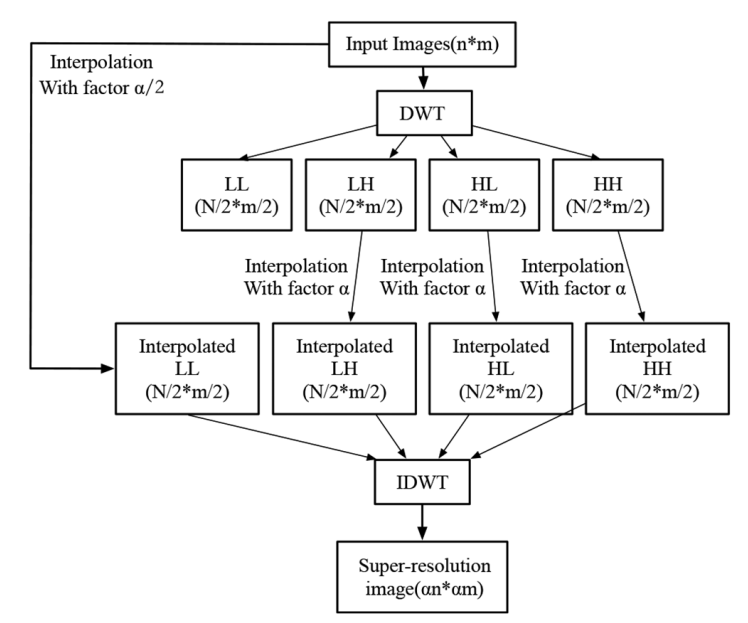
\includegraphics[width=0.75\textwidth]{images/dwt-method}
                \caption{Flowchart of DWT and BI method}
                \label{fig:dwt-method}
                \end{figure}
            }
        \end{frame}
    \end{section}
    \begin{section}{CNN Based Methods}
        \begin{frame}
            \frametitle{CNN}
            A convolutional neural network (CNN) is a type of artificial neural network used primarily for image recognition and processing,
            due to its ability to recognize patterns in images~\cite{armcnn}
            \begin{figure}
                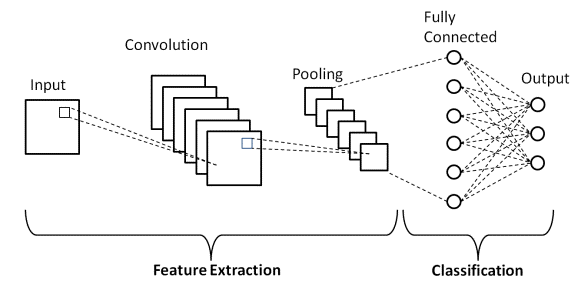
\includegraphics[width=0.75\textwidth]{images/cnn}
                \caption{Basic CNN Architecture~\cite{ugcnn}}
                \label{fig:cnn-arch}
            \end{figure}
        \end{frame}
        \begin{frame}
            \frametitle{Convolution Layer}
            This type of layer is used to \textbf{extract features} from the input images.
            The output is termed as the Feature map which gives us information about the image such as the corners and edges.
            \begin{figure}
                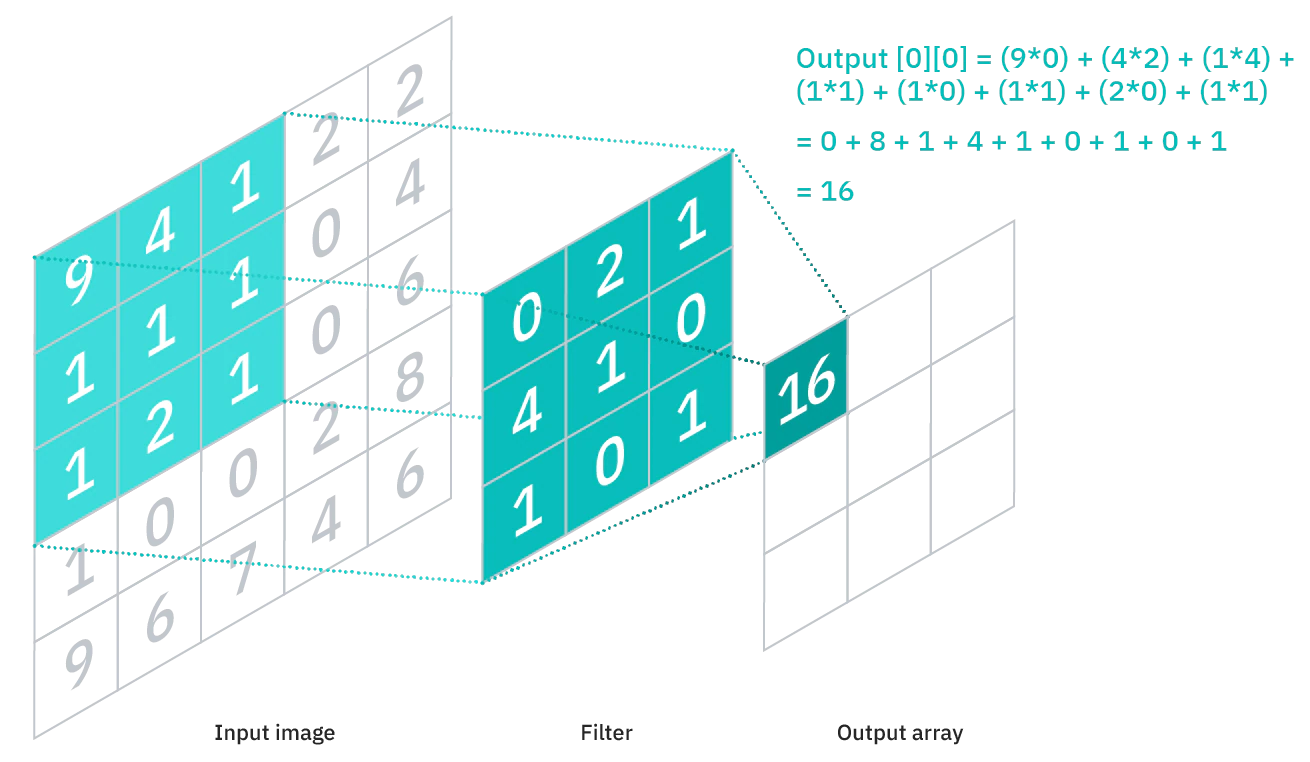
\includegraphics[width=0.6\textwidth]{images/conv-layer}
                \caption{Basic CNN Architecture~\cite{ugcnn}}
                \label{fig:conv-layer}
            \end{figure}
        \end{frame}
        \begin{frame}[label=cnn-list]
            \frametitle{CNN Models}
            Most important CNN based models for Image Super Resolution:
            \begin{itemize}
                \item SRCNN
                \item EDSR
                \item WDSR
                \item RDN
                \item DSRN
                \item LRFNet
                \item RCAN
                \item CARN
                \item IDN
            \end{itemize}
        \end{frame}
        \begin{frame}
            \frametitle{SRCNN}
            \only<1>{SRCNN is the pioneering work of deep learning applications
            in the field of super-resolution reconstruction.
            SRCNN's structure is very simple, using only three convolution layers.}
            \only<2>{
                For a given LR image, it uses the bicubic algorithm to zoom to
                the target size first and then run
                that through the three convolution layers:
            }
            \only<2>{\begin{enumerate}
            \item Feature extraction and representation
            \item Non-linear mapping
            \item Reconstruction
            \end{enumerate}}
            \only<3>{
                SRCNN uses MSE as a loss function, which is beneficial to
                obtain a higher PSNR.

                \vfill

                \hfill$ L_{MSE}=\frac{1}{n}\sum_{i=1}^{n}\left\| F(Y_{i}-X_{i})\right\|^2 $\hfill
            }
            \only<1>{
                \begin{figure}
                \centering
                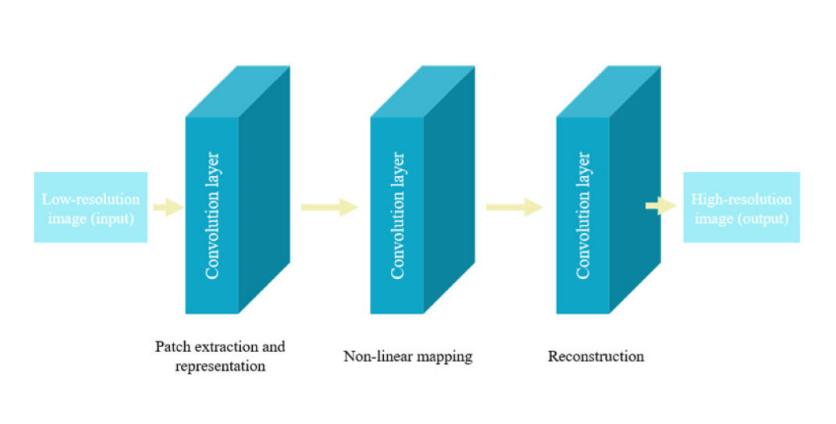
\includegraphics[width=0.75\textwidth]{images/srcnn-struct}
                \caption{SRCNN structure~\cite{li2020}}
                \label{fig:srcnn-struct}
                \end{figure}
            }
            \only<2>{
                \begin{figure}
                \centering
                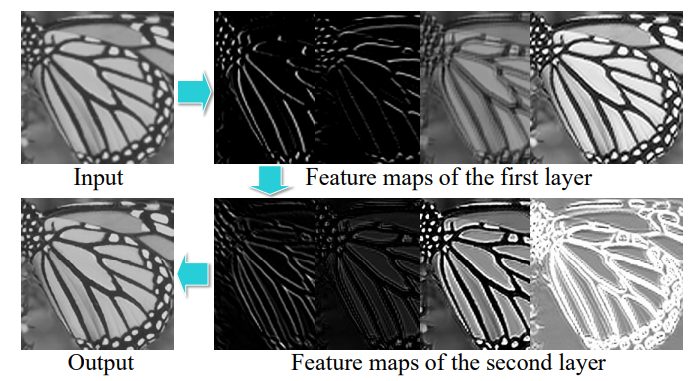
\includegraphics[width=0.75\textwidth]{images/srcnn-layers}
                \caption{Example feature maps of different layers~\cite{srcnn}}
                \label{fig:srcnn-layers}
                \end{figure}
            }
        \end{frame}
        \begin{frame}
            \frametitle{EDSR}
            The network structure of EDSR is based on the improvement of SRResNet.
            The batch normalisation (BN) layer in the residual block is removed, and the ReLU active layer is not set outside the
            residual block.
            \begin{figure}
                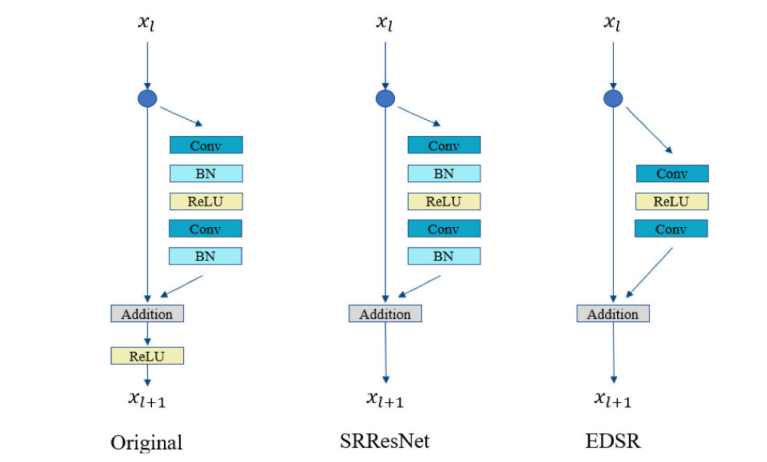
\includegraphics[width=0.75\textwidth]{images/edsr-srresnet-rb}
                \caption{Comparison of the original, SRResNet and EDSR residual blocks}
                \label{fig:edsr-srresnet-rb}
            \end{figure}
        \end{frame}
        \begin{frame}
            \frametitle{EDSR}
            \only<1>{
                Since the BN layer consumes the same amount of memory as the convolutional layer.
                removing it means that EDSR can stack more network layers
                or extract more features for each layer for better performance with
                the same computing resources.
            }
            \only<2>{
                EDSR uses the $ L_{1}$ loss function to optimise the network model:

                \vfill

                \hfill$ L_{1}\left( P \right)=\frac{1}{N}\sum_{p\in P}^{}\left| x(p)-y(p)\right|$\hfill
            }
            \only<1>{
                \begin{figure}
                \centering
                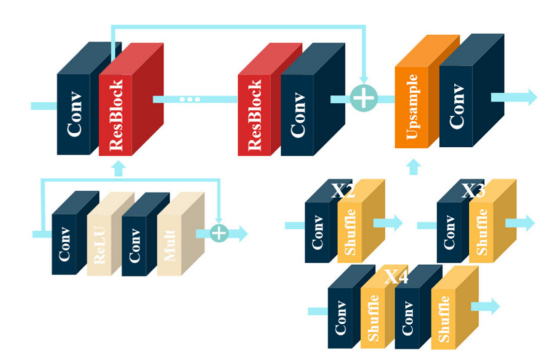
\includegraphics[width=0.55\textwidth]{images/edsr-struct}
                \caption{Network structure of EDSR}
                \label{fig:edsr-struct}
                \end{figure}
            }
        \end{frame}
        \againframe{cnn-list}
        % dense blocks - cancading
    \end{section}
    \begin{section}{GAN Based Models}
        \begin{frame}
            \frametitle{GAN}
            A \textbf{generative adversarial network} consists of Two neural networks
            that contest with each other in the form of a zero-sum game, where one agent's gain is another agent's loss.
            \begin{figure}
                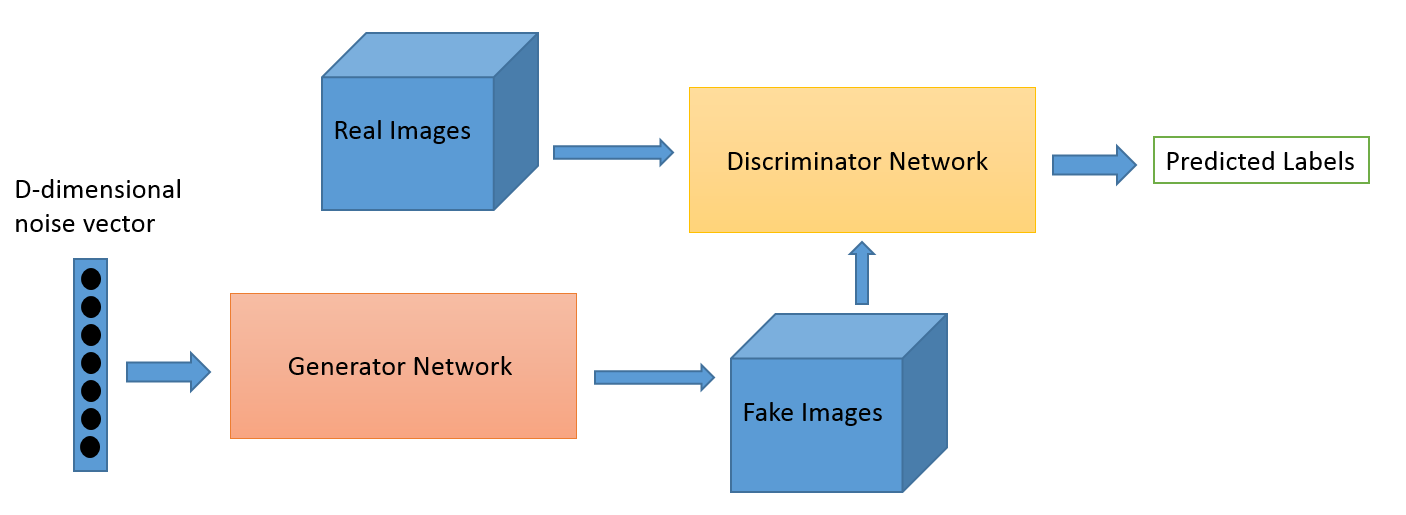
\includegraphics[width=0.8\textwidth]{images/gan_schema}
                \caption{discriminator-generator feedback loop~\cite{pmgan}}
                \label{fig:gan-schema}
            \end{figure}
        \end{frame}
        \begin{frame}[label=gan-list]
            \frametitle{GAN Models}
            \begin{itemize}
                \item SRGAN
                \item ESRGAN
                \item ProSR
                \item CinCycle
                \item SRFeat
            \end{itemize}
        \end{frame}
        \begin{frame}
            \frametitle{SRGAN}
            \only<1>{
                This network is the first framework to recover 4× down-sampled images.
                Here is the architecture of generator and discriminator network~\cite{li2020}: }
            \only<2>{
                The structure also modified the loss function from the mean squared
                loss function to a
                new \textcolor{blue}{\textbf{perceptual loss}} function consisting of resistance loss and
                content loss.
            }
            \only<1>{
                \begin{figure}
                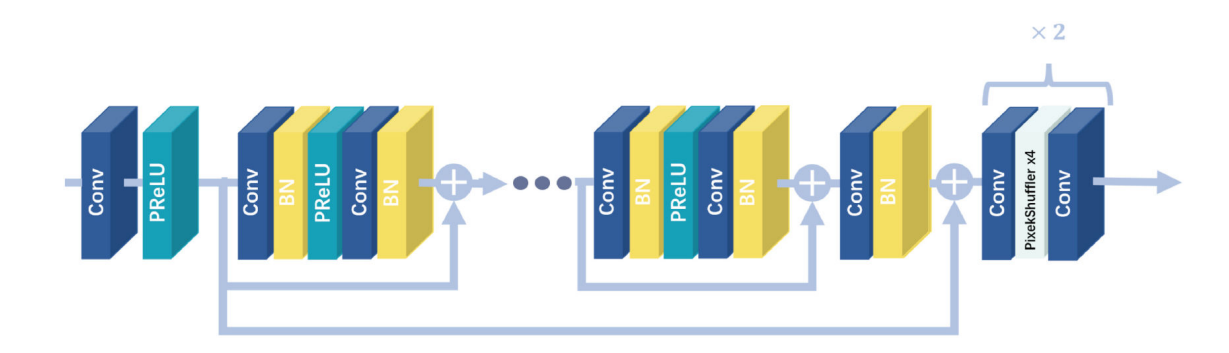
\includegraphics[width=0.75\textwidth]{images/srgan-gen}
                \caption{Generation network structure of SRGAN~\cite{li2020}}
                \label{fig:srgan-generator}
                \end{figure}
                \begin{figure}
                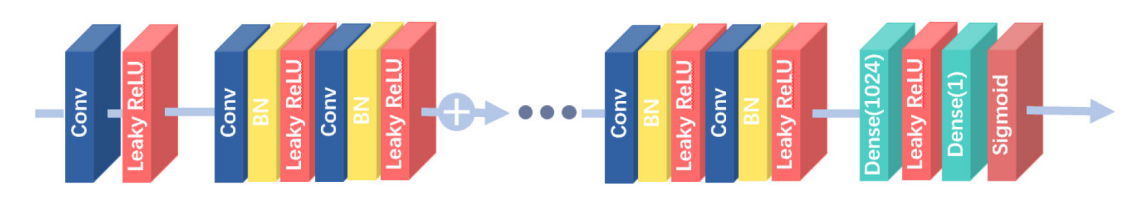
\includegraphics[width=0.75\textwidth]{images/srgan-dis}
                \caption{Discriminant network structure of SRGAN~\cite{li2020}}
                \label{fig:srgan-discriminator}
                \end{figure}


%                \begin{figure}
%                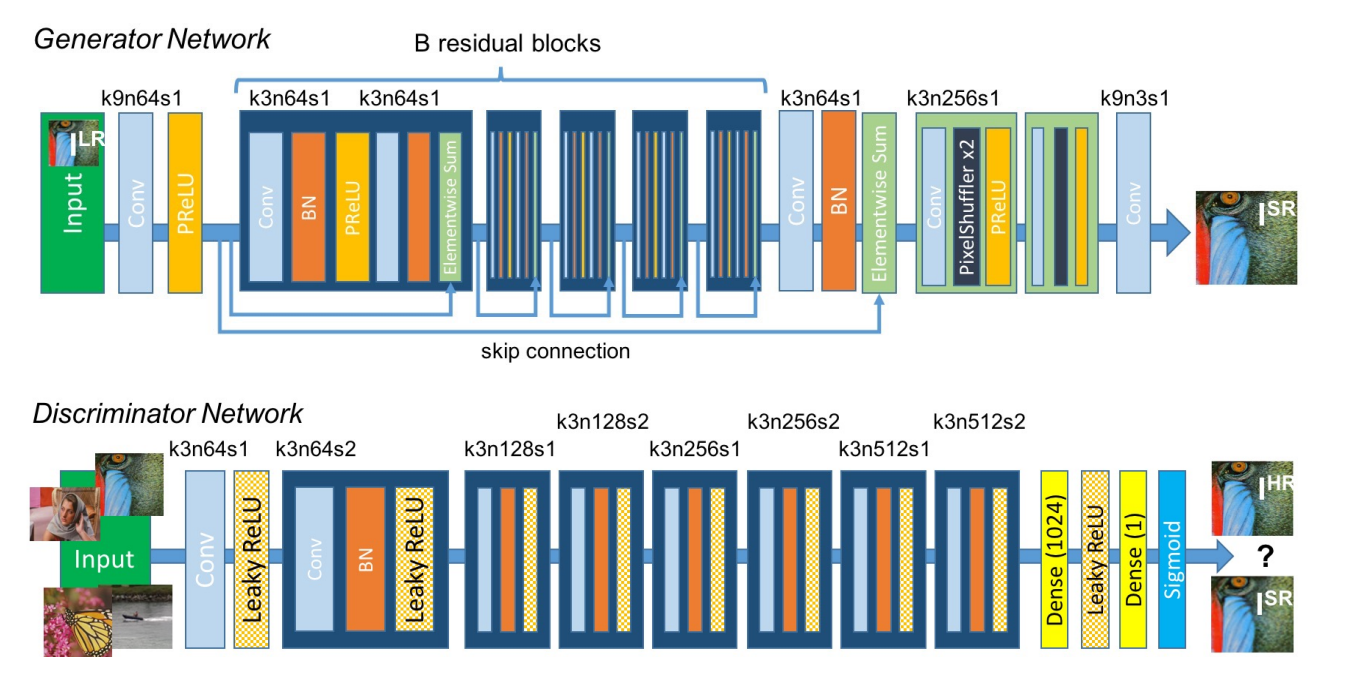
\includegraphics[width=\textwidth]{images/srgan-arch}
%                \label{fig:srgan-arch}
%                \end{figure}
            }
            \only<3>{
                An example photo-realistic image that was super resolved
                with a 4× upscaling factor is shown below with corresponding PSNR and SSIM are shown in brackets~\cite{th2016}:
            }
            \only<3>{
                \begin{figure}
                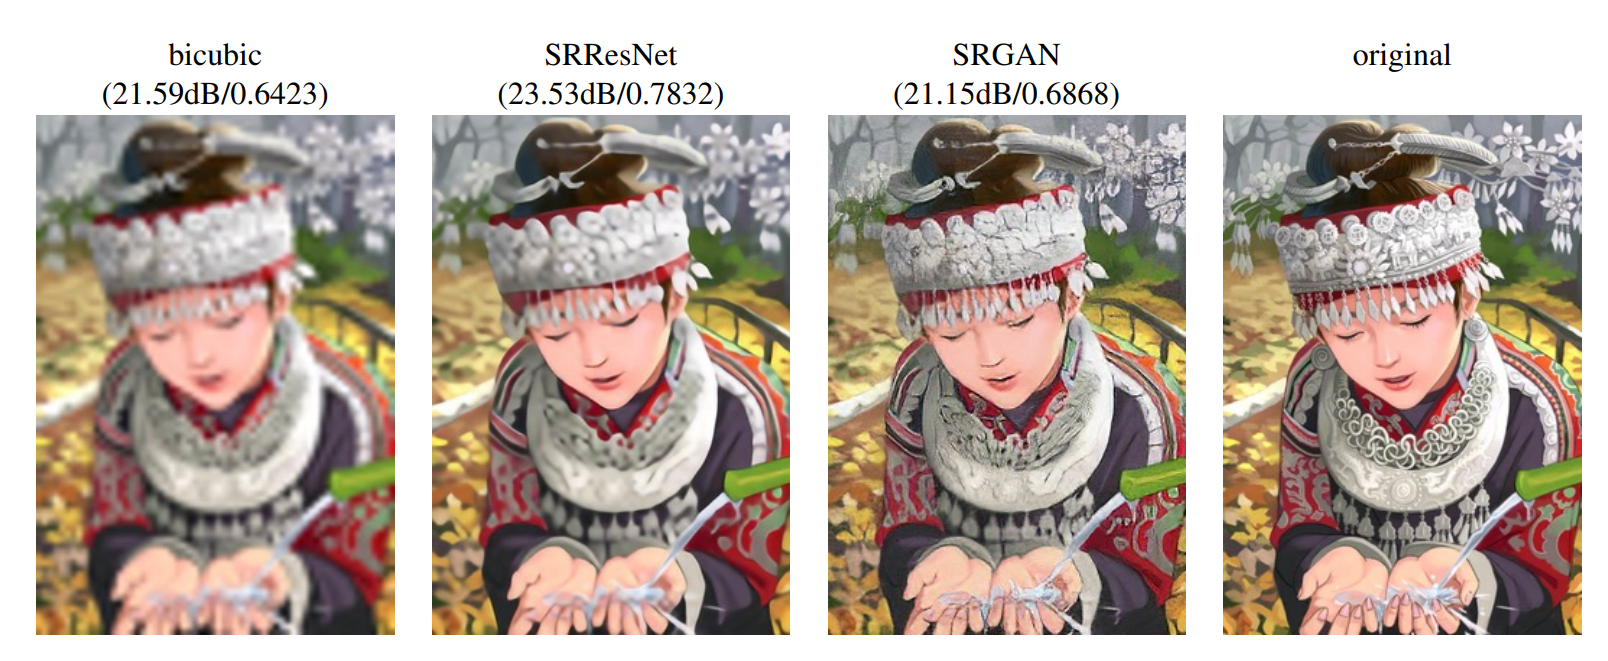
\includegraphics[width=\textwidth]{images/srgan-comparison}
                \label{fig:srgan-comparison}
                \end{figure}
            }
        \end{frame}
        \begin{frame}
            \frametitle{ESRGAN}
            ESRGAN is a model proposed based on the improvement of SRGAN.
            it aims to improve the three key parts of SRGAN:
            \begin{itemize}
                \item Network Structure
                \item Adversarial Loss
                \item Perceived Loss
            \end{itemize}

        \end{frame}
        \begin{frame}
            \frametitle{ESRGAN - Network Structure}
            First, the the BN layers in residual blocks from SRGAN are removed:
            \begin{figure}
                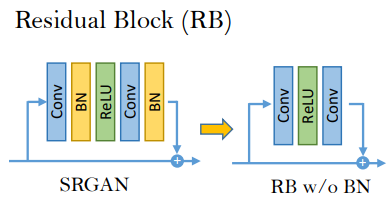
\includegraphics[width=0.5\textwidth]{images/esrgan-rb}
                \caption{New Residual Block Structure~\cite{wang2018}}
                \label{fig:esrgan-rb}
            \end{figure}
        \end{frame}
        \begin{frame}
            \frametitle{ESRGAN - Network Structure}
            Second, RRDB block is used in our deeper model and $\beta$ is the residual scaling parameter:
            \begin{figure}
                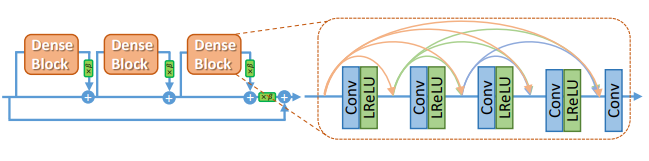
\includegraphics[width=0.8\textwidth]{images/esrgan-rrdb}
                \caption{Residual in Residual Dense Block~\cite{wang2018}}
                \label{fig:esrgan-rrdb}
            \end{figure}
        \end{frame}
        \begin{frame}
            \frametitle{ESRGAN - Adversarial Loss}
            which estimates the probability that one input image $x$ is real and
            natural, a relativistic discriminator tries to predict the probability that a real
            image $x_{r}$ is relatively more realistic than a fake one $x_{f}$
            \begin{figure}
                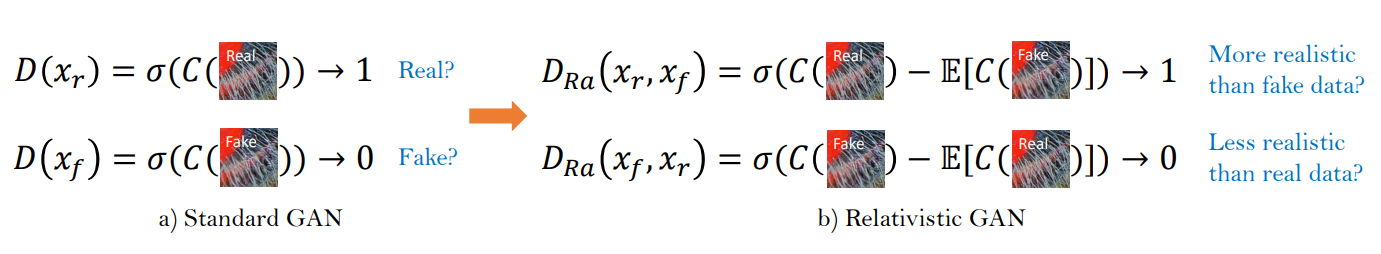
\includegraphics[width=0.8\textwidth]{images/esrgan-discriminator}
                \caption{Difference between standard discriminator and relativistic discriminator~\cite{wang2018}}
                \label{fig:esrgan-discriminator}
            \end{figure}
        \end{frame}
        \begin{frame}
            \frametitle{ESRGAN - Perceived Loss}
            ESRGAN proposes a more efficient perceptual domain loss,
            using pre-activation features.
            This will overcome two shortcomings:
            \begin{enumerate}
                \item Sparse activated features
                \item Remove inconsistent reconstructed brightness compared with the ground-truth image
            \end{enumerate}
        \end{frame}
        \begin{frame}
            \frametitle{ESRGAN}
            \begin{figure}
                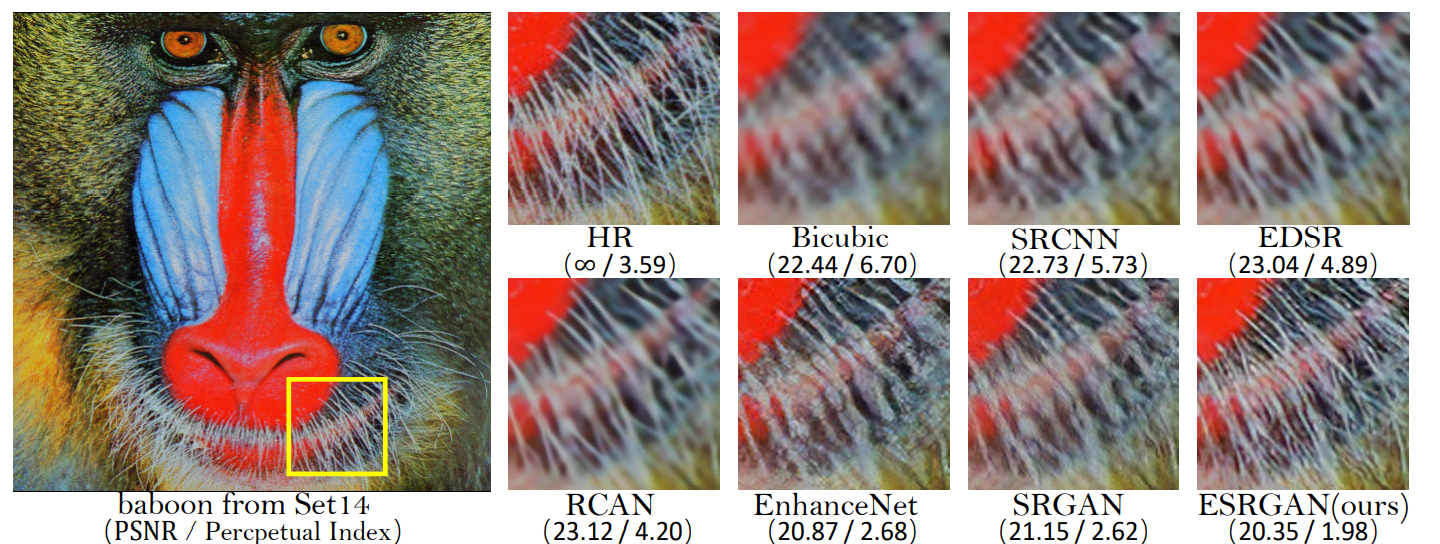
\includegraphics[width=\textwidth]{images/esrgan-baboon}
                \caption{ESRGAN produces more natural textures~\cite{wang2018}}
                \label{fig:esrgan-comparison}
            \end{figure}
        \end{frame}
        \againframe{gan-list}
    \end{section}
    \begin{frame}
        \frametitle{Conclusion}
        \begin{itemize}
            \item Evaluation indexes: PSNR, SSIM, PI and RMSE
            \item Interpolation-based SR: BI-based, DWT-based
            \item CNN-based SR: SRCNN, EDSR, \ldots
            \item GAN-based SR: SRGAN, ESRGAN, \ldots
        \end{itemize}
    \end{frame}
    \begin{frame}[t, allowframebreaks]
        \frametitle{References}
        \bibliographystyle{plain}
        \bibliography{refs}
    \end{frame}
    \begin{frame}[standout]
	Thank you for your attention!
        %\centering \LARGE
        %\emph{Thank you for your attention!}
    \end{frame}
\end{document}